% Options for packages loaded elsewhere
\PassOptionsToPackage{unicode}{hyperref}
\PassOptionsToPackage{hyphens}{url}
%
\documentclass[
]{book}
\usepackage{amsmath,amssymb}
\usepackage{lmodern}
\usepackage{iftex}
\ifPDFTeX
  \usepackage[T1]{fontenc}
  \usepackage[utf8]{inputenc}
  \usepackage{textcomp} % provide euro and other symbols
\else % if luatex or xetex
  \usepackage{unicode-math}
  \defaultfontfeatures{Scale=MatchLowercase}
  \defaultfontfeatures[\rmfamily]{Ligatures=TeX,Scale=1}
\fi
% Use upquote if available, for straight quotes in verbatim environments
\IfFileExists{upquote.sty}{\usepackage{upquote}}{}
\IfFileExists{microtype.sty}{% use microtype if available
  \usepackage[]{microtype}
  \UseMicrotypeSet[protrusion]{basicmath} % disable protrusion for tt fonts
}{}
\makeatletter
\@ifundefined{KOMAClassName}{% if non-KOMA class
  \IfFileExists{parskip.sty}{%
    \usepackage{parskip}
  }{% else
    \setlength{\parindent}{0pt}
    \setlength{\parskip}{6pt plus 2pt minus 1pt}}
}{% if KOMA class
  \KOMAoptions{parskip=half}}
\makeatother
\usepackage{xcolor}
\usepackage{color}
\usepackage{fancyvrb}
\newcommand{\VerbBar}{|}
\newcommand{\VERB}{\Verb[commandchars=\\\{\}]}
\DefineVerbatimEnvironment{Highlighting}{Verbatim}{commandchars=\\\{\}}
% Add ',fontsize=\small' for more characters per line
\usepackage{framed}
\definecolor{shadecolor}{RGB}{248,248,248}
\newenvironment{Shaded}{\begin{snugshade}}{\end{snugshade}}
\newcommand{\AlertTok}[1]{\textcolor[rgb]{0.94,0.16,0.16}{#1}}
\newcommand{\AnnotationTok}[1]{\textcolor[rgb]{0.56,0.35,0.01}{\textbf{\textit{#1}}}}
\newcommand{\AttributeTok}[1]{\textcolor[rgb]{0.77,0.63,0.00}{#1}}
\newcommand{\BaseNTok}[1]{\textcolor[rgb]{0.00,0.00,0.81}{#1}}
\newcommand{\BuiltInTok}[1]{#1}
\newcommand{\CharTok}[1]{\textcolor[rgb]{0.31,0.60,0.02}{#1}}
\newcommand{\CommentTok}[1]{\textcolor[rgb]{0.56,0.35,0.01}{\textit{#1}}}
\newcommand{\CommentVarTok}[1]{\textcolor[rgb]{0.56,0.35,0.01}{\textbf{\textit{#1}}}}
\newcommand{\ConstantTok}[1]{\textcolor[rgb]{0.00,0.00,0.00}{#1}}
\newcommand{\ControlFlowTok}[1]{\textcolor[rgb]{0.13,0.29,0.53}{\textbf{#1}}}
\newcommand{\DataTypeTok}[1]{\textcolor[rgb]{0.13,0.29,0.53}{#1}}
\newcommand{\DecValTok}[1]{\textcolor[rgb]{0.00,0.00,0.81}{#1}}
\newcommand{\DocumentationTok}[1]{\textcolor[rgb]{0.56,0.35,0.01}{\textbf{\textit{#1}}}}
\newcommand{\ErrorTok}[1]{\textcolor[rgb]{0.64,0.00,0.00}{\textbf{#1}}}
\newcommand{\ExtensionTok}[1]{#1}
\newcommand{\FloatTok}[1]{\textcolor[rgb]{0.00,0.00,0.81}{#1}}
\newcommand{\FunctionTok}[1]{\textcolor[rgb]{0.00,0.00,0.00}{#1}}
\newcommand{\ImportTok}[1]{#1}
\newcommand{\InformationTok}[1]{\textcolor[rgb]{0.56,0.35,0.01}{\textbf{\textit{#1}}}}
\newcommand{\KeywordTok}[1]{\textcolor[rgb]{0.13,0.29,0.53}{\textbf{#1}}}
\newcommand{\NormalTok}[1]{#1}
\newcommand{\OperatorTok}[1]{\textcolor[rgb]{0.81,0.36,0.00}{\textbf{#1}}}
\newcommand{\OtherTok}[1]{\textcolor[rgb]{0.56,0.35,0.01}{#1}}
\newcommand{\PreprocessorTok}[1]{\textcolor[rgb]{0.56,0.35,0.01}{\textit{#1}}}
\newcommand{\RegionMarkerTok}[1]{#1}
\newcommand{\SpecialCharTok}[1]{\textcolor[rgb]{0.00,0.00,0.00}{#1}}
\newcommand{\SpecialStringTok}[1]{\textcolor[rgb]{0.31,0.60,0.02}{#1}}
\newcommand{\StringTok}[1]{\textcolor[rgb]{0.31,0.60,0.02}{#1}}
\newcommand{\VariableTok}[1]{\textcolor[rgb]{0.00,0.00,0.00}{#1}}
\newcommand{\VerbatimStringTok}[1]{\textcolor[rgb]{0.31,0.60,0.02}{#1}}
\newcommand{\WarningTok}[1]{\textcolor[rgb]{0.56,0.35,0.01}{\textbf{\textit{#1}}}}
\usepackage{longtable,booktabs,array}
\usepackage{calc} % for calculating minipage widths
% Correct order of tables after \paragraph or \subparagraph
\usepackage{etoolbox}
\makeatletter
\patchcmd\longtable{\par}{\if@noskipsec\mbox{}\fi\par}{}{}
\makeatother
% Allow footnotes in longtable head/foot
\IfFileExists{footnotehyper.sty}{\usepackage{footnotehyper}}{\usepackage{footnote}}
\makesavenoteenv{longtable}
\usepackage{graphicx}
\makeatletter
\def\maxwidth{\ifdim\Gin@nat@width>\linewidth\linewidth\else\Gin@nat@width\fi}
\def\maxheight{\ifdim\Gin@nat@height>\textheight\textheight\else\Gin@nat@height\fi}
\makeatother
% Scale images if necessary, so that they will not overflow the page
% margins by default, and it is still possible to overwrite the defaults
% using explicit options in \includegraphics[width, height, ...]{}
\setkeys{Gin}{width=\maxwidth,height=\maxheight,keepaspectratio}
% Set default figure placement to htbp
\makeatletter
\def\fps@figure{htbp}
\makeatother
\setlength{\emergencystretch}{3em} % prevent overfull lines
\providecommand{\tightlist}{%
  \setlength{\itemsep}{0pt}\setlength{\parskip}{0pt}}
\setcounter{secnumdepth}{5}
\usepackage{booktabs}
\ifLuaTeX
  \usepackage{selnolig}  % disable illegal ligatures
\fi
\usepackage[]{natbib}
\bibliographystyle{plainnat}
\IfFileExists{bookmark.sty}{\usepackage{bookmark}}{\usepackage{hyperref}}
\IfFileExists{xurl.sty}{\usepackage{xurl}}{} % add URL line breaks if available
\urlstyle{same} % disable monospaced font for URLs
\hypersetup{
  pdftitle={AIS: Capacitación de R},
  pdfauthor={Oliab Herrera Coria},
  hidelinks,
  pdfcreator={LaTeX via pandoc}}

\title{AIS: Capacitación de R}
\author{Oliab Herrera Coria}
\date{2023-02-08}

\begin{document}
\maketitle

{
\setcounter{tocdepth}{1}
\tableofcontents
}
\hypertarget{informaciuxf3n-del-curso}{%
\chapter*{Información del curso}\label{informaciuxf3n-del-curso}}
\addcontentsline{toc}{chapter}{Información del curso}

\begin{itemize}
\item
  Este es un curso de Introducción a R.
\item
  Al final serán capaces de utilizar R para cargar datos, arreglarlos, hacer gráficos y tablas, e informes en Rmarkdown.
\item
  Intentaremos que el curso sea fundamentalmente práctico.
\item
  En lugar de presentar todos los pormenores de R de manera lineal, se irán presentando distintos aspectos de R conforme se vayan necesitando; es decir, no vamos a presentar R como un lenguaje de programación sino como una herramienta para hacer análisis estadísticos.
\end{itemize}

E- n la carpeta del curso están todos los materiales: tutoriales, algunos datos, etc\ldots.

\hypertarget{ligas}{%
\subsubsection*{Ligas}\label{ligas}}
\addcontentsline{toc}{subsubsection}{Ligas}

Notas:\\
Correo: \href{mailto:oliabherrera@gmail.com}{\nolinkurl{oliabherrera@gmail.com}}

\hypertarget{temario}{%
\section*{Temario}\label{temario}}
\addcontentsline{toc}{section}{Temario}

\begin{enumerate}
\def\labelenumi{\arabic{enumi}.}
\tightlist
\item
  \textbf{Introducción a R}
\end{enumerate}

\begin{itemize}
\tightlist
\item
  Instalación de R y R Studio.
\item
  Entorno de trabajo de RStudio.
\item
  Instalación de paquetes.
\item
  Ayuda en R.
\end{itemize}

\begin{enumerate}
\def\labelenumi{\arabic{enumi}.}
\setcounter{enumi}{1}
\tightlist
\item
  \textbf{Manipulación y visualización de datos}
\end{enumerate}

\begin{itemize}
\tightlist
\item
  Visualización de datos.
\item
  Manipulación y limpieza de datos.
\item
  Temas selectos de programación en R.
\end{itemize}

\begin{enumerate}
\def\labelenumi{\arabic{enumi}.}
\setcounter{enumi}{2}
\tightlist
\item
  \textbf{Reportes POS}
\end{enumerate}

\begin{itemize}
\tightlist
\item
  Descarga de datos.
\item
  Scripts principales.
\item
  Proyecciones.
\end{itemize}

\hypertarget{software}{%
\subsection*{Software}\label{software}}
\addcontentsline{toc}{subsection}{Software}

\begin{itemize}
\tightlist
\item
  \url{https://www.r-project.org}
\item
  \url{https://www.rstudio.com}
\end{itemize}

\hypertarget{introducciuxf3n-a-r.}{%
\chapter{Introducción a R.}\label{introducciuxf3n-a-r.}}

El objetivo de este tutorial es familiarizarnos con el entorno de trabajo que proporciona R y RStudio. Al finalizar este tutorial también deberemos ser capaces de instalar y cargar los paquetes que vayamos a necesitar para realizar nuestros análisis de datos.

\hypertarget{instalaciuxf3n-de-r-y-r-studio.}{%
\section{Instalación de R y R Studio.}\label{instalaciuxf3n-de-r-y-r-studio.}}

Para instalar R vamos a la página web de R project: \url{http://www.r-project.org}

\begin{figure}
\centering
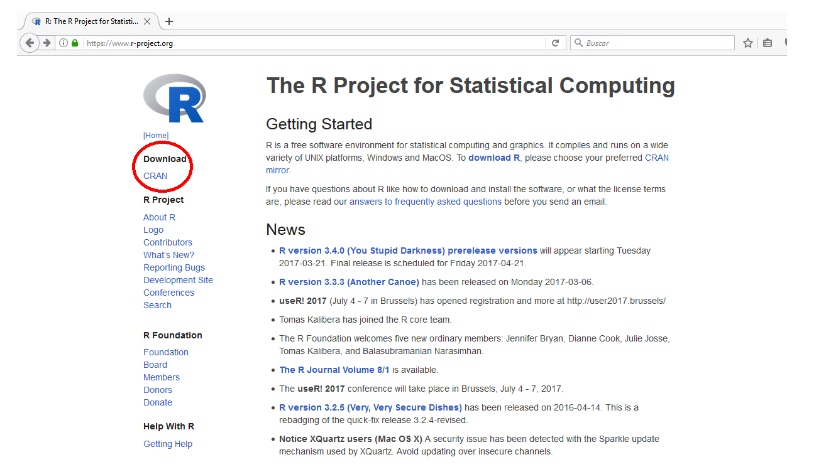
\includegraphics{imagenes/01.png}
\caption{Figura 1}
\end{figure}

Para descargar la aplicación hacemos clic en Cran y pinchamos sobre el enlace del ``espejo'' más próximo a nuestra ubicación, México. Seleccionemos la URL de, por ejemplo (\url{https://cran.itam.mx/}).

\begin{figure}
\centering
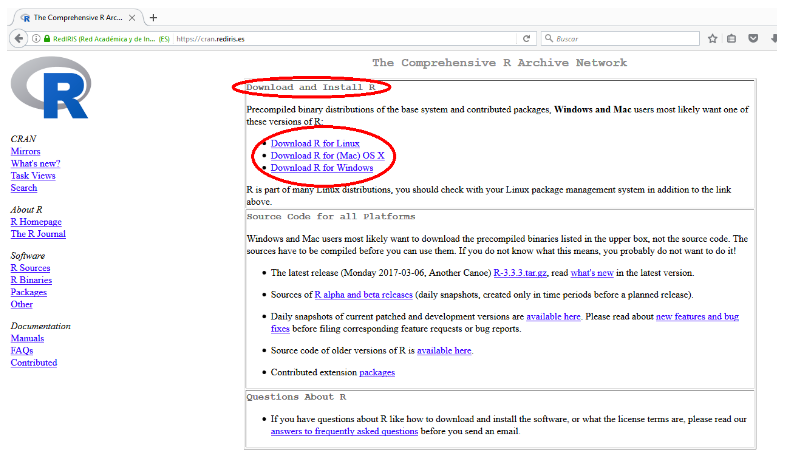
\includegraphics{imagenes/02.png}
\caption{Figura 2}
\end{figure}

Ahora, en función del tu sistema operativo, seleccionar la correspondiente opción.

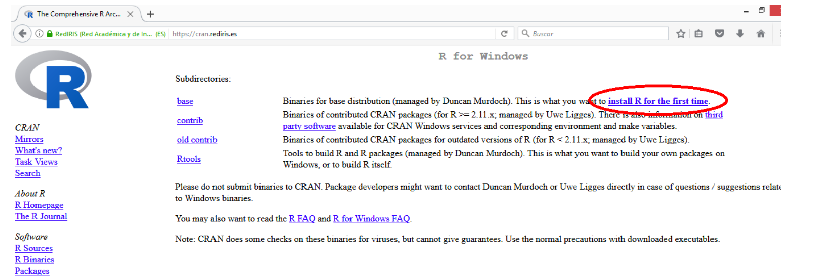
\includegraphics{imagenes/03.png}
\#\#\# Instalar R en Windows.

Al hacer clic sobre Download R for Windows iremos a la página que se reproduce más abajo. Hacer clic sobre \emph{install R for the first time.}

En la siguiente ventana, hacer clic sobre \emph{Download R 3.3.3 for Windows} y guardar el archivo de instalación.

Ejecutar el archivo descargado para proceder a la instalación de R.

\hypertarget{instalar-r-en-mac.}{%
\subsection{Instalar R en Mac.}\label{instalar-r-en-mac.}}

Al hacer clic sobre Download R for (Mac) OS X iremos a la página que se reproduce más abajo. Hacer clic sobre install R for the first time.

\begin{figure}
\centering
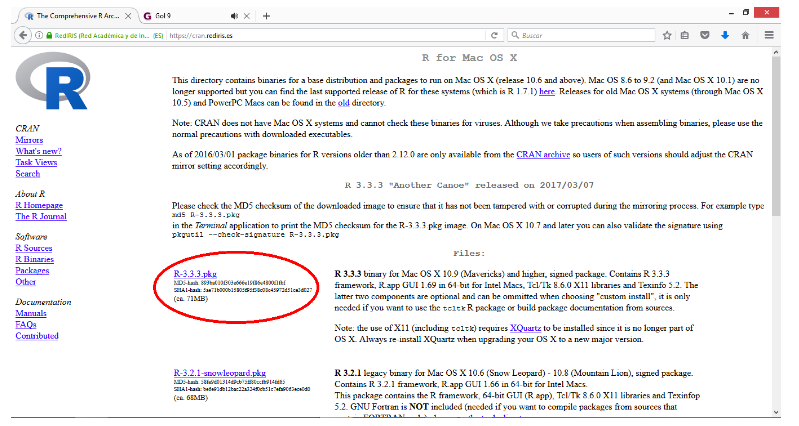
\includegraphics{imagenes/04.png}
\caption{Figura 4}
\end{figure}

Hacer clic sobre R-3.3.3.pkg y guardar el archivo de instalación. Ejecutar el archivo descargado para proceder a la instalación de R.

\hypertarget{instalar-rstudio}{%
\subsection{Instalar RStudio}\label{instalar-rstudio}}

Descargamos la aplicación desde la página web de RStudio \href{https://posit.co/download/rstudio-desktop/}{aquí} según nuestra plataforma de trabajo:

\begin{itemize}
\item
  RStudio 1.0.136 - Windows Vista/7/8/10.
\item
  RStudio 1.0.136 - Mac OS X 10.6+ (64-bit).
\end{itemize}

Una vez guardado el archivo, lo ejecutamos para instalar RStudio. Sigue las instrucciones de instalación.

\hypertarget{entorno-de-trabajo-de-rstudio.}{%
\section{Entorno de trabajo de RStudio.}\label{entorno-de-trabajo-de-rstudio.}}

En general trabajamos con la interfaz de RStudio antes que con la de R porque la primera es ``más amigable''.

Si abrimos RStudio vamos a ver algo parecido a lo que se muestra en la siguiente imagen:

\begin{figure}
\centering
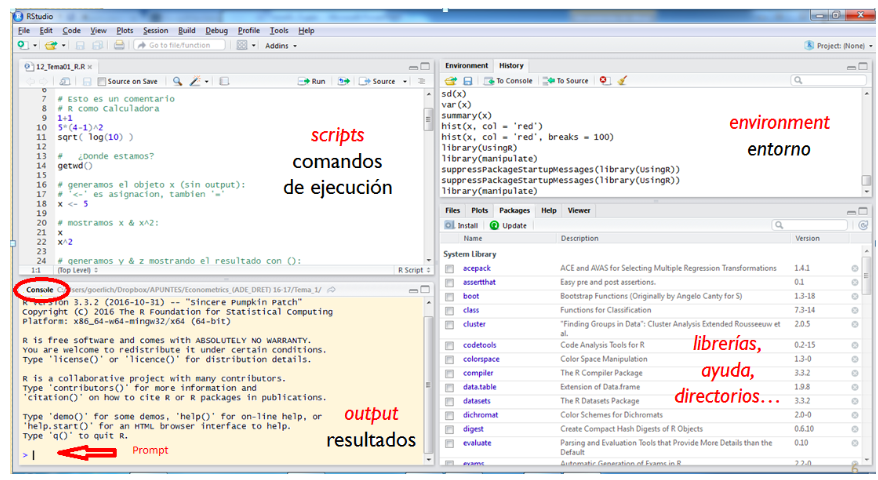
\includegraphics{imagenes/05.png}
\caption{Figura 5}
\end{figure}

Una vez estamos en RStudio, podemos escribir y ejecutar las órdenes de varias formas:

\begin{itemize}
\item
  directamente en la consola.
\item
  a través de un script (.R).
\item
  con ficheros Rmarkdown (.Rmd).
\end{itemize}

Como podemos ver, RStudio está (normalmente) dividido en 4 paneles.

\hypertarget{consola}{%
\subsection{Consola}\label{consola}}

Por defecto, la consola se encuentra en el panel inferior-izquierdo. ¿Vemos la pestaña que pone Console? Inmediatamente debajo aparece un texto informativo y, finalmente, el símbolo ``\textgreater{}''. Aquí es donde R espera que le demos instrucciones. Para ejecutarlas y obtener el resultado pulsamos enter.

Vamos a hacer este ejemplo:

\begin{Shaded}
\begin{Highlighting}[]
\DecValTok{2}\SpecialCharTok{+}\DecValTok{2}
\end{Highlighting}
\end{Shaded}

\begin{verbatim}
## [1] 4
\end{verbatim}

\begin{Shaded}
\begin{Highlighting}[]
\DecValTok{5}\SpecialCharTok{*}\NormalTok{(}\DecValTok{3{-}1}\NormalTok{)}\SpecialCharTok{\^{}}\DecValTok{2}
\end{Highlighting}
\end{Shaded}

\begin{verbatim}
## [1] 20
\end{verbatim}

\begin{Shaded}
\begin{Highlighting}[]
\FunctionTok{sqrt}\NormalTok{(}\DecValTok{4}\NormalTok{)}
\end{Highlighting}
\end{Shaded}

\begin{verbatim}
## [1] 2
\end{verbatim}

\hypertarget{scripts}{%
\subsection{Scripts}\label{scripts}}

Trabajar en la consola es muy limitado ya que las instrucciones se han de introducir una a una. Lo habitual es trabajar con scripts o ficheros de instrucciones. Estos ficheros tienen extensión \textbf{.R}.

Se puede crear una script con cualquier editor de texto (uno de los más populares es Tinn-R), pero nosotros lo haremos desde RStudio. Para ello, seleccionamos la siguiente ruta de menús: \textbf{File \textgreater{} New File \textgreater{} R script}

\begin{figure}
\centering
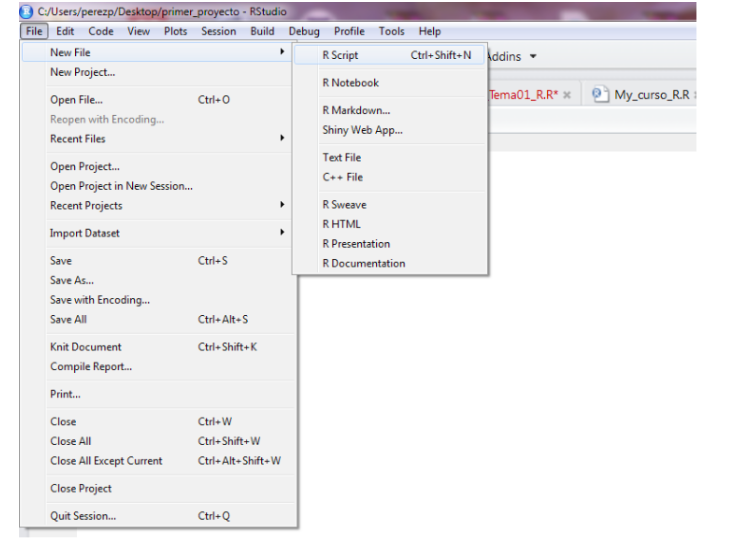
\includegraphics{imagenes/06.png}
\caption{Figura 5}
\end{figure}

El panel del script se sitúa en la parte superior-izquierda de RStudio. Ahora podemos escribir las instrucciones línea por línea. Las instrucciones las podemos ejecutar una a una o las podemos seleccionar y ejecutar en bloque. Para ejecutar las instrucciones tenemos varias alternativas:

\begin{itemize}
\item
  Hacemos clic en el botón: \textbf{Run} (botón situado en la parte derecha de las opciones del panel de script)
\item
  Pulsamos Ctrl+r
\item
  Ejecutamos el código desde las opciones del menú Code. Sinceramente, esto nunca lo hemos utilizado. ¡Cuestión de comodidad!
\end{itemize}

Como se muestra en la imagen más abajo, vamos a escribir nuestro primer script.

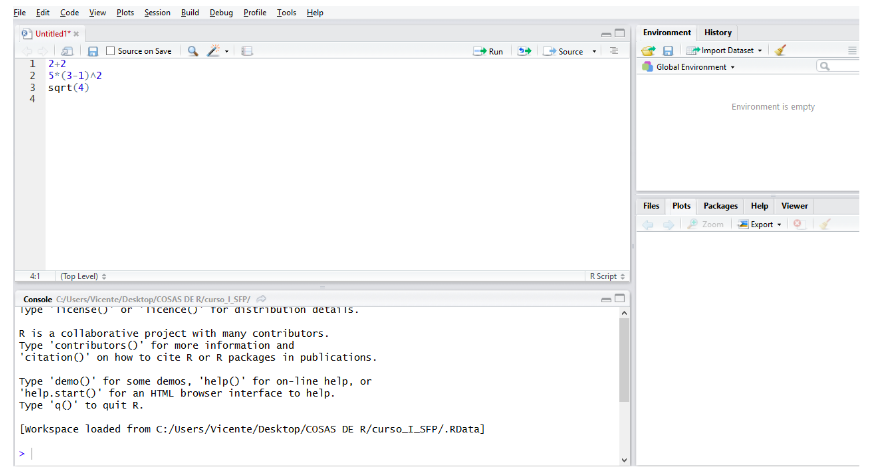
\includegraphics{imagenes/07.png}
Para guardar el script:

\begin{itemize}
\item
  File \textgreater{} Save as.. y seleccionar la ruta donde se quiere guardar el fichero.
\item
  Hacer clic en el botón Guardar que se encuentra en la parte izquierda de la cinta de opciones del script.
\end{itemize}

\hypertarget{entorno}{%
\subsection{Entorno}\label{entorno}}

El panel, llamémoslo, de entorno esta compuesto de dos pestañas: Environment y History.

\begin{itemize}
\tightlist
\item
  En el Environment se irán registrando los objetos que vayamos creando en la sesión de trabajo. También tenemos la opción de cargar y guardar una sesión de trabajo, importar datos y limpiar los objetos de la sesión. Estas opciones están accesibles a través de la cinta de opciones de la pestaña.
\end{itemize}

\begin{figure}
\centering
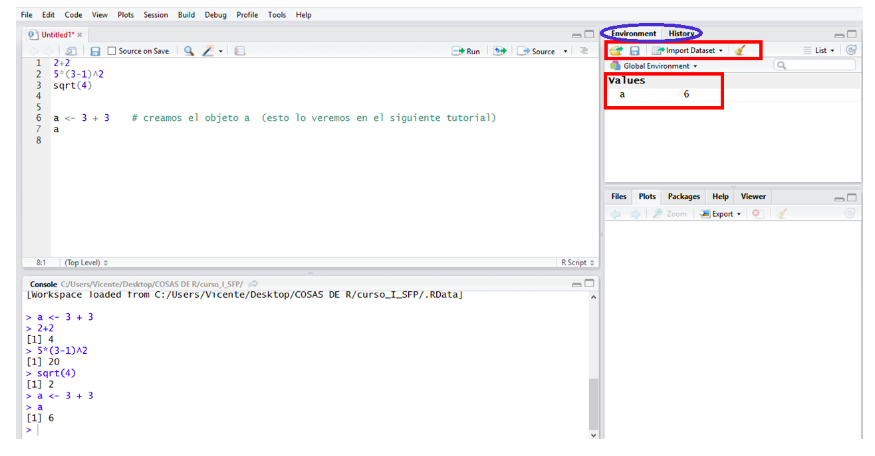
\includegraphics{imagenes/08.png}
\caption{Figura 7}
\end{figure}

\begin{itemize}
\tightlist
\item
  En la pestaña History se registran las instrucciones ejecutadas. Como opciones, podemos cargar y guardar el historial de la sesión, seleccionar una o más instrucciones y enviarlas bien a la consola bien al script, y limpiar el historial.
\end{itemize}

\hypertarget{otros-recursos}{%
\subsection{Otros recursos}\label{otros-recursos}}

Con el nombre de \textbf{Otros recursos} nos referimos al panel que se encuentra en la parte inferior-derecha del escritorio de RStudio. ¡No sabía cómo llamarlo!

En este panel cabe destacar las siguientes pestañas, cada una con diferentes opciones:

\begin{itemize}
\item
  Files: es una especie de explotador de ficheros.
\item
  Plots: donde se visualizan los gráficos que creamos. Entre las opciones disponibles se encuentran:
\item
  Zoom: para agrandar el gráfico y verlo en otra ventana.
\item
  Export: para exportar/guardar el gráfico. Se puede guardar el gráfico como imagen, pdf o copiarlo al portapapeles.
\item
  Packages: proporciona un listado de los paquetes instalados en R y los que han sido cargado en la sesión. A través de las opciones de esta pestaña podemos instalar nuevos paquetes o actualizar los existentes.
\item
  Help: Para obtener ayuda sobre una determinada función.
\end{itemize}

\hypertarget{instalaciuxf3n-de-paquetes.}{%
\section{Instalación de paquetes.}\label{instalaciuxf3n-de-paquetes.}}

\hypertarget{ayuda-en-r.}{%
\section{Ayuda en R.}\label{ayuda-en-r.}}

\hypertarget{prueba}{%
\chapter{Prueba}\label{prueba}}

\hypertarget{aqui-va-ora-cosa}{%
\section{Aqui va ora cosa}\label{aqui-va-ora-cosa}}

  \bibliography{book.bib,packages.bib}

\end{document}
